\textsc{\huge Используемые структуры}
\begin{lstlisting}[caption={\text{Структура open\_flags}}]
struct open_flags {
	int open_flag;
	umode_t mode;
	int acc_mode;
	int intent;
	int lookup_flags;
};
\end{lstlisting}

\begin{lstlisting}[caption={\text{Структура filename}}]
struct filename {
	const char		*name;	/* pointer to actual string */
	const __user char	*uptr;	/* original userland pointer */
	int			refcnt;
	struct audit_names	*aname;
	const char		iname[];
};	
\end{lstlisting}

\begin{lstlisting}[caption={\text{Структура nameidata}}]
struct nameidata {
	struct path	path;
	struct qstr	last;
	struct path	root;
	struct inode	*inode; /* path.dentry.d_inode */
	unsigned int	flags, state;
	unsigned	seq, m_seq, r_seq;
	int		last_type;
	unsigned	depth;
	int		total_link_count;
	struct saved {
		struct path link;
		struct delayed_call done;
		const char *name;
		unsigned seq;
	} *stack, internal[EMBEDDED_LEVELS];
	struct filename	*name;
	struct nameidata *saved;
	unsigned	root_seq;
	int		dfd;
	kuid_t		dir_uid;
	umode_t		dir_mode;
} __randomize_layout;	
\end{lstlisting}

\textsc{\huge Схемы алгоритмов} \\
\begin{figure}[H]
	\centering
	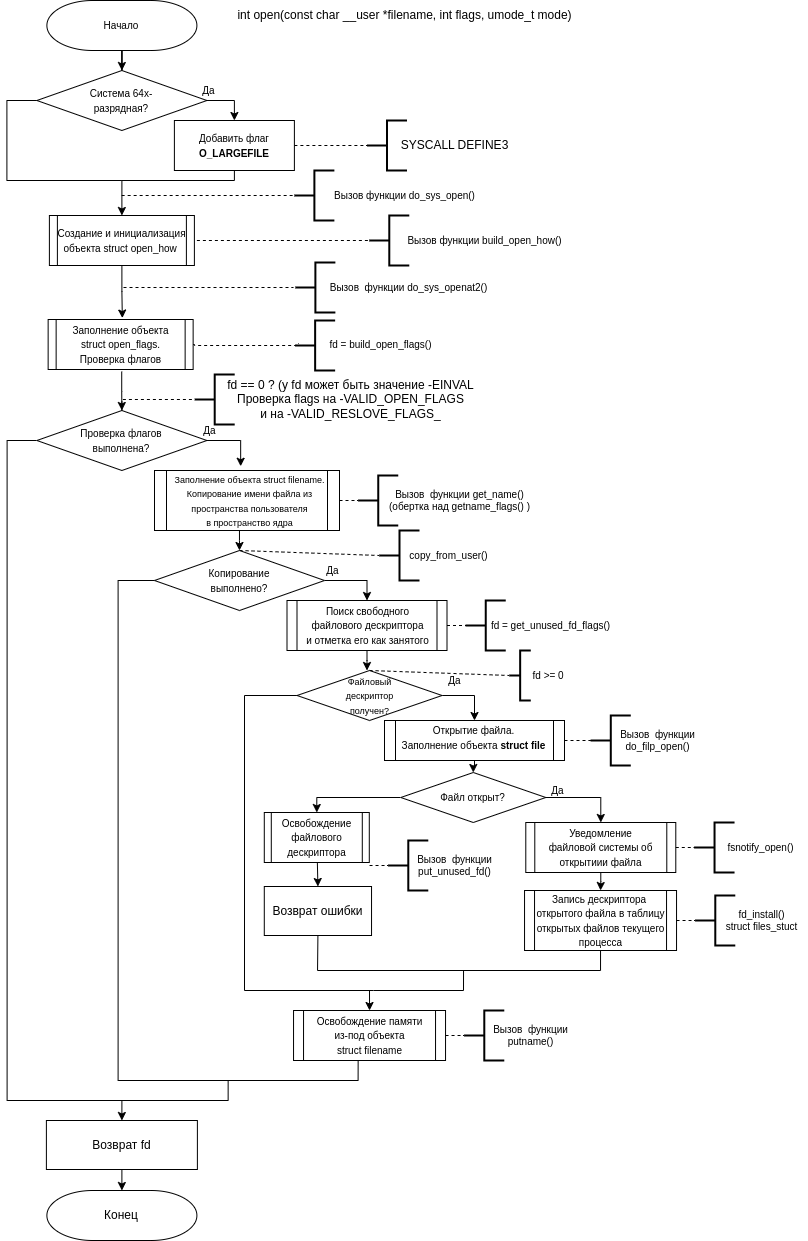
\includegraphics[scale=0.5]{assets/open-open.drawio.png}
	\caption{Схема алгоритма работы системного вызова open()}
\end{figure}

\begin{figure}[H]
	\centering
	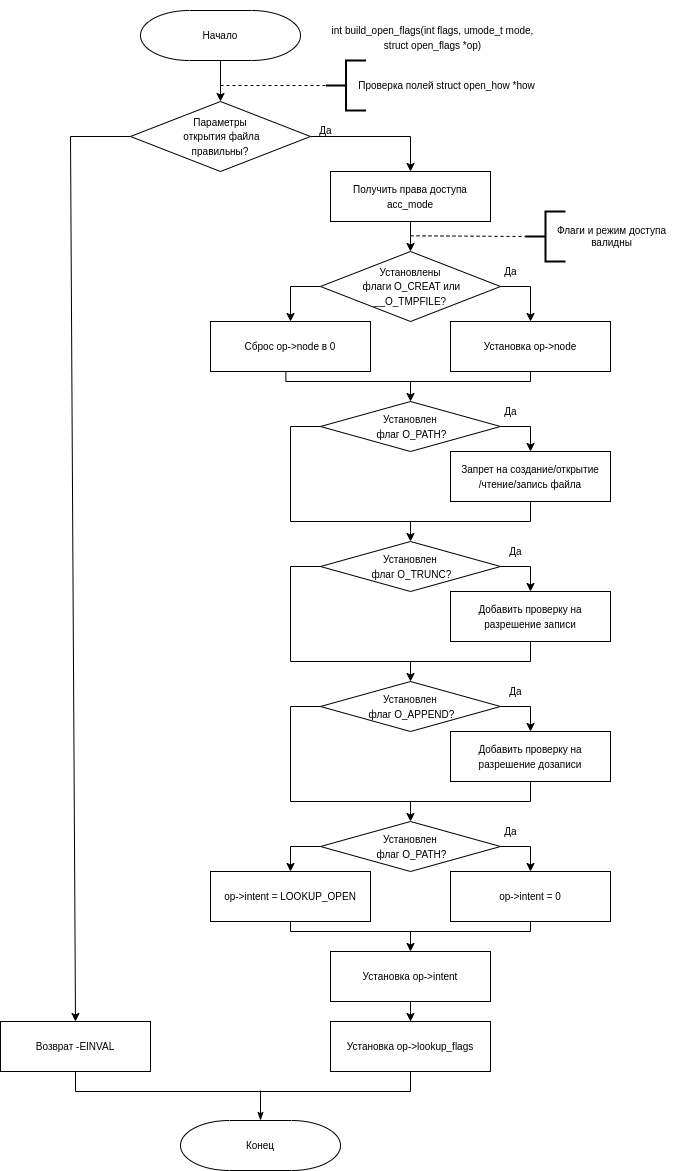
\includegraphics[scale=0.6]{assets/open-build_open_flags.drawio.png}
	\caption{Схема алгоритма работы функции build\_open\_flags()}
\end{figure}

\begin{figure}[H]
	\centering
	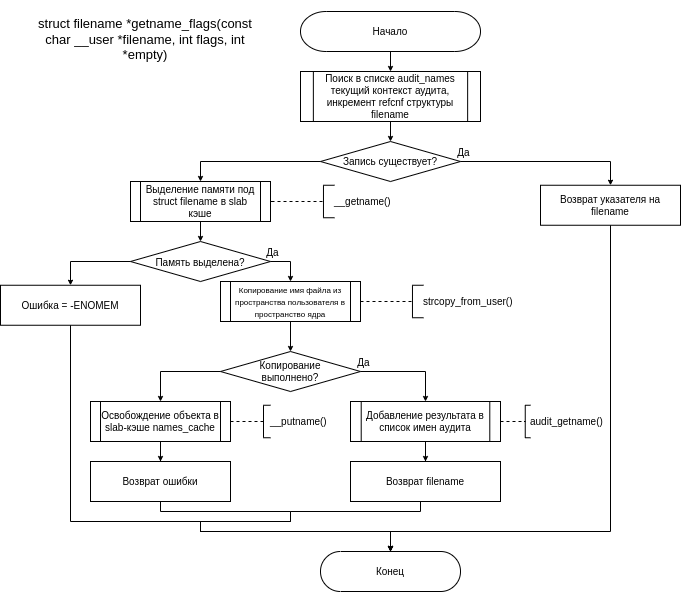
\includegraphics[scale=0.7]{assets/open-getname_flags.drawio.png}
	\caption{Схема алгоритма работы функции getname\_flags()}
\end{figure}

\begin{figure}[H]
	\centering
	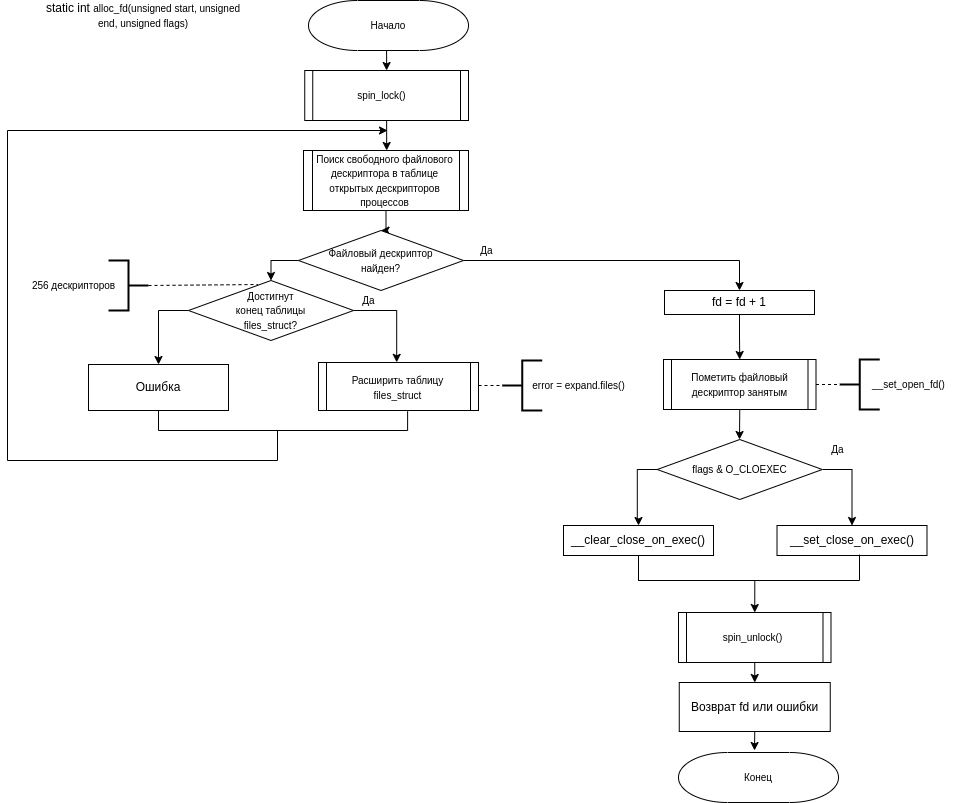
\includegraphics[scale=0.47]{assets/open-alloc_fd.drawio.png}
	\caption{Схема алгоритма работы функции alloc\_fd()}
\end{figure}

\begin{figure}[H]
	\centering
	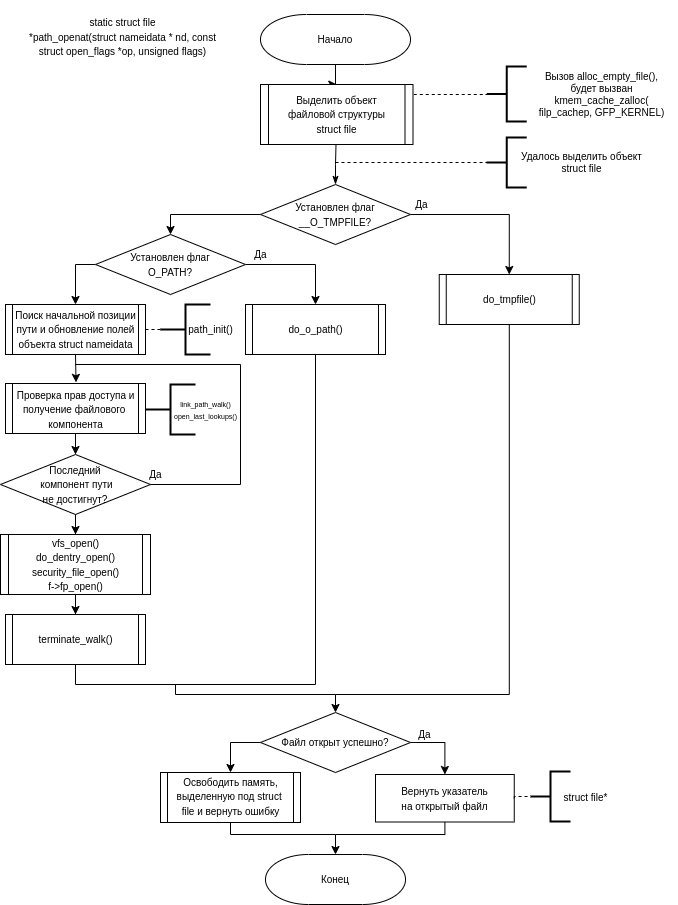
\includegraphics[scale=0.6]{assets/open-path_openat.drawio.png}
	\caption{Схема алгоритма функции path\_openat()}
\end{figure}

\begin{figure}[H]
	\centering
	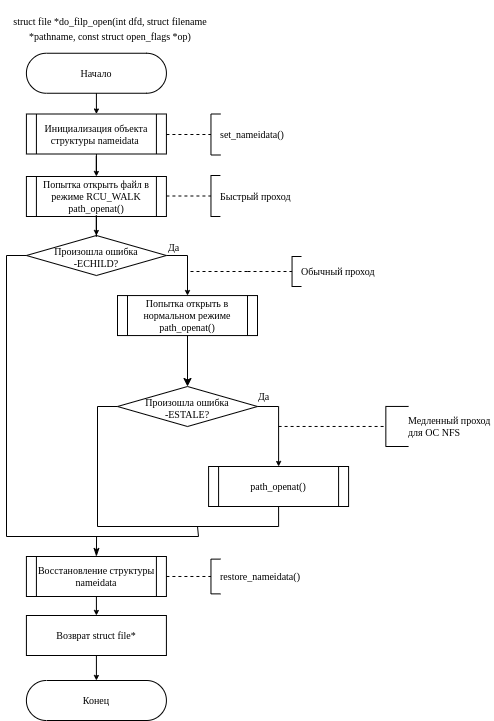
\includegraphics[scale=0.8]{assets/open-do_filp_open.drawio.png}
	\caption{Схема алгоритмов функций, работающих с nameidata (do filp open)}
\end{figure}

\begin{figure}[H]
	\centering
	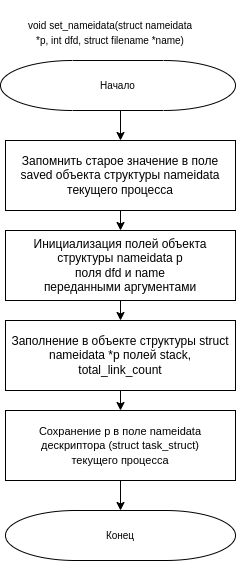
\includegraphics[scale=0.8]{assets/open-set_nameidata.drawio.png}
	\caption{Схема алгоритмов функций, работающих с nameidata}
\end{figure}

LOOKUP\_RCU --- флаг для открытия файла в режиме RCU\_walk (Допускает
возможность одновременного доступа).

LOOKUP\_REVAL --- флаг для ФС NFS O\_APPEND.

O\_APPEND может проводить к потери данных файлов в ФС NFS,
если одновременно добавл. данные нескольких процессов.
Нельзя избежать ускорение гонки.

NFS не поддерживает добавление в файл, потому клиентское ядро имитирует такое поведение.

\begin{figure}[H]
	\centering
	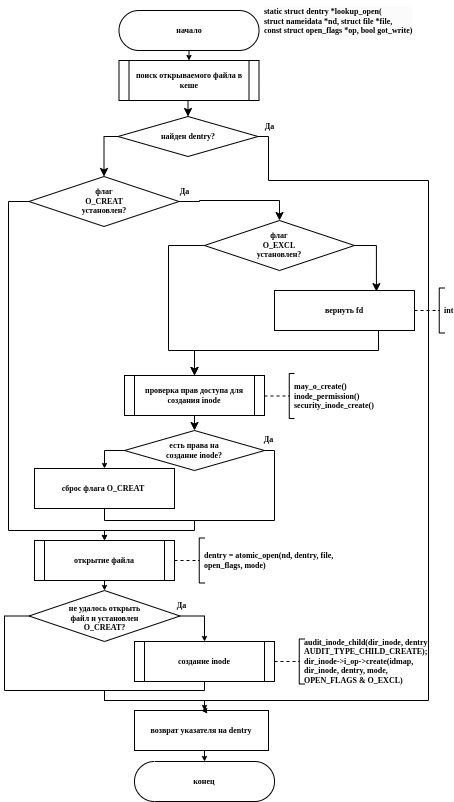
\includegraphics[scale=0.6]{assets/open-lookup_open.drawio.png}
	\caption{Схема алгоритма функции open\_last\_lookups()}
\end{figure}

\begin{figure}[H]
	\centering
	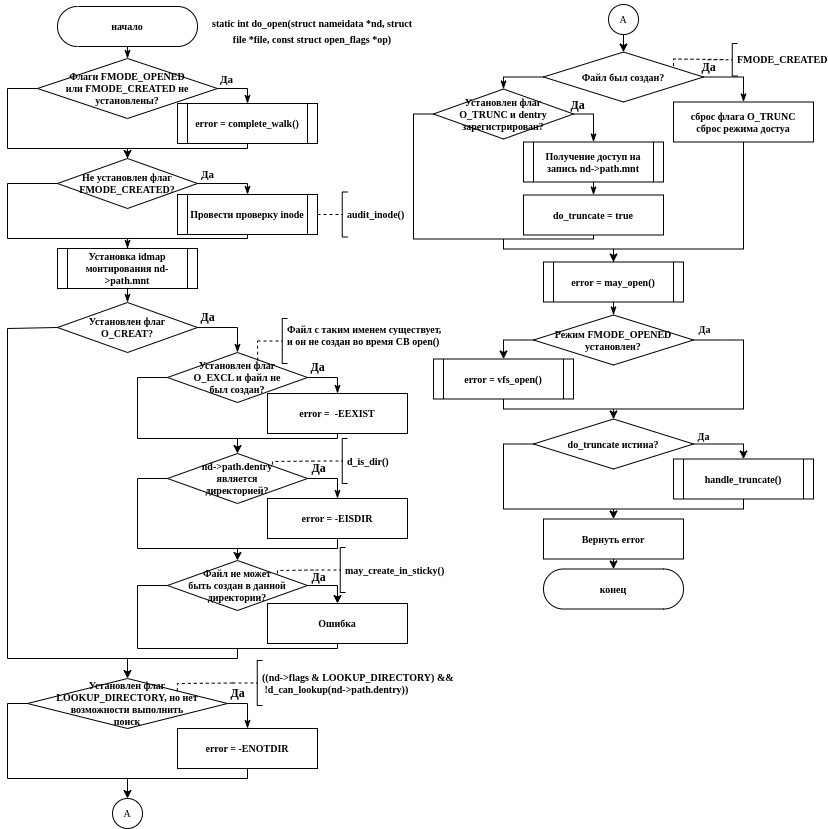
\includegraphics[scale=0.6]{assets/lab06-do_open.drawio.png}
	\caption{Схема алгоритма функции do\_open() начало}
\end{figure}

\begin{figure}[H]
	\centering
	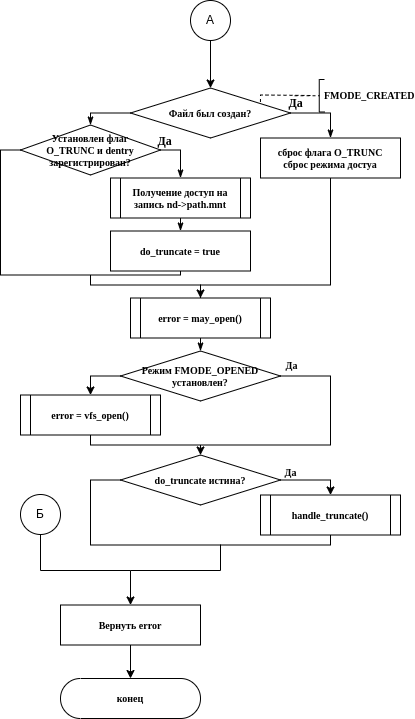
\includegraphics[scale=0.7]{assets/lab06 (2)-do_open_2.drawio.png}
	\caption{Схема алгоритма функции do\_open() продолжение}
\end{figure}
\begin{figure}[H]
	\centering
	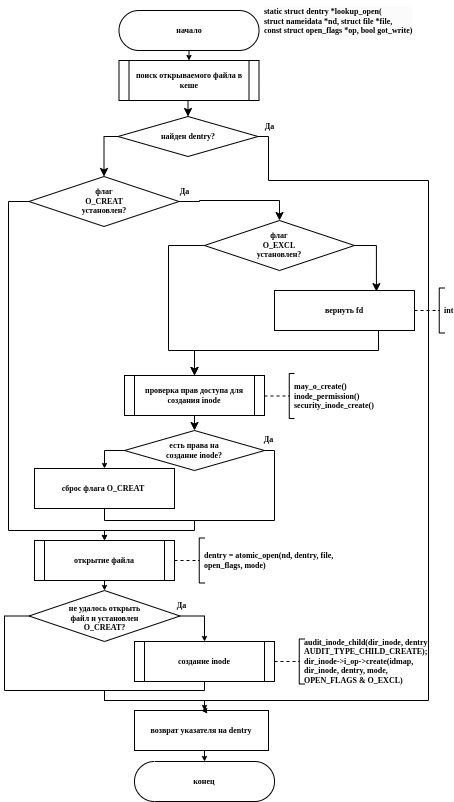
\includegraphics[scale=0.65]{assets/open-lookup_open.drawio.png}
	\caption{Схема алгоритма функции open\_lookup()}
\end{figure}

\begin{figure}[H]
	\centering
	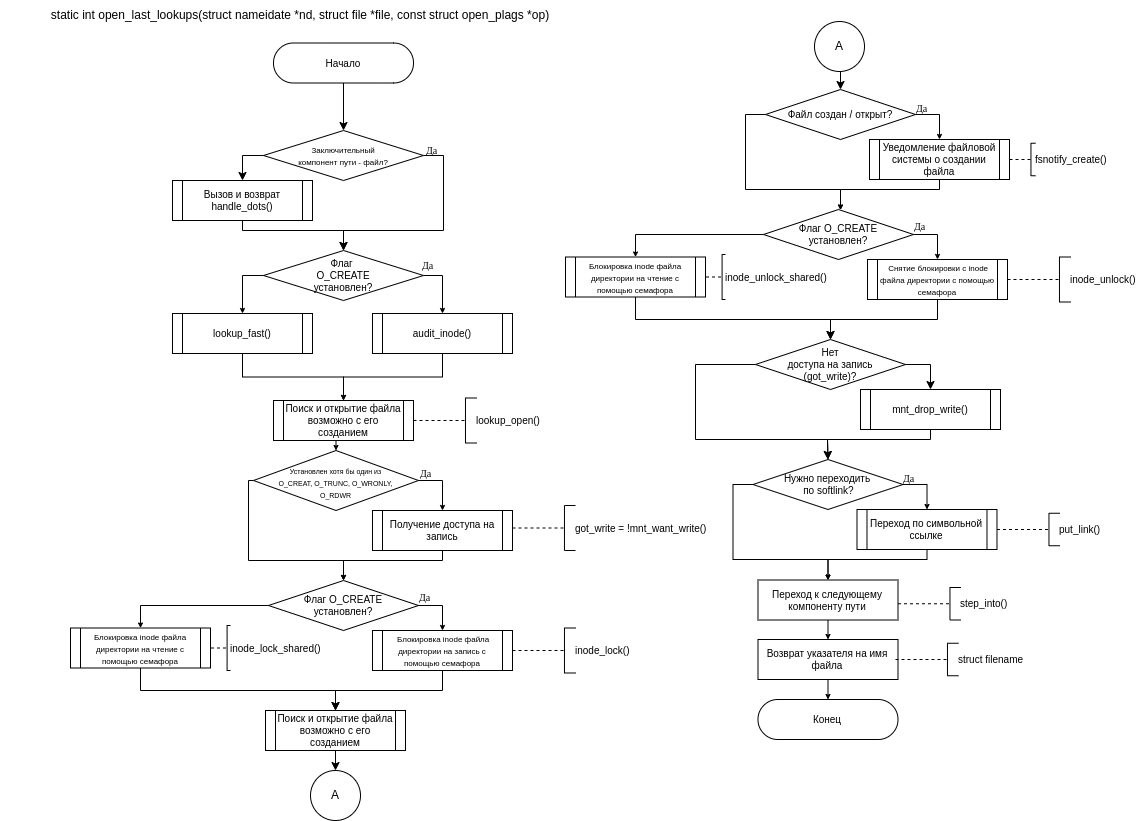
\includegraphics[scale=0.47]{assets/open-open_last_lookups.drawio.png}
	\caption{Схема алгоритма функции last\_lookup()}
\end{figure}